\section{I/O Automata Programming Model\label{representation}}

In this section, we show how I/O automata can be used to construct programs.
To motivate the presentation, we develop an automaton for electing a leader in a unidirectional ring using the LCR algorithm.

\subsection{I/O Automata Representation}

\paragraph{Leader election in a unidirectional ring.}
Nodes in a distributed system are arranged in a ring so that two consecutive nodes are connected by a channel.
The goal is to designate one of the nodes as the leader of the ring.
The solution we adopt is the asynchronous LCR algorithm presented by Lynch in Chapter 15 of~\cite{lynch1996distributed} which is in turn based on the work of LeLann~\cite{le1977distributed} and Chang and Roberts~\cite{chang1979improved}.
The LCR algorithm assumes that every node has a unique identifier (UID).
When the protocol begins, each node sends its UID to its successor.
When a node receives a UID from its predecessor that is greater than its own UID, it forwards the UID to its successor.
When a node receives its own UID, it elects itself the leader of the ring.
Our implementation of the asynchronous LCR automaton is located in \verb+examples/asynch_lcr_automaton.hpp+ of the ioa++ package.

\paragraph{Declaring an automaton.}
All automata inherit from the common base class \verb+ioa::automaton+ which implements the system action interface.
The following code declares the \verb+asynch_lcr_automaton+:
\begin{lstlisting}
template <typename UID>
class asynch_lcr_automaton :
  public virtual ioa::automaton
{
  ...
};
\end{lstlisting}
Static composition can be accomplished by inheriting from, i.e., extending, other automata.
A problem arises when an automaton extends more than one automaton since the common \verb+ioa::automaton+ base class will be duplicated for each inheritance path.
The solution is to make the \verb+ioa::automaton+ base class a virtual base class which eliminates the duplicates and resolves all references appropriately.
The \verb+asynch_lcr_automaton+ is declared as a template where the type \verb+UID+ is the type used for unique identifiers.
This makes the \verb+asynch_lcr_automaton+ general since it can use any type that models the unique identifier concept.

\paragraph{Declaring and initializing state variables.}
The state variables of an automaton are expressed as member variables.
The \verb+asynch_lcr_automaton+ has four state variables containing the unique id of the automaton, a queue of outgoing messages, and flags for reporting a change in status:
\begin{lstlisting}
private:
  const UID m_u;
  std::queue<UID> m_send;
  bool m_report;
  bool m_leader;
\end{lstlisting}
Notice that the member variables are declared \verb+private+ which is in keeping with the notion that the state of each automaton is independent.
State variables are initialized using a constructor.
For the \verb+asynch_lcr_automaton+, the id is initialized, the send queue contains the id of the automaton, the automaton does not need to report its leader status, and the automaton is not the leader:
\begin{lstlisting}
public:
  asynch_lcr_automaton (const UID& u) :
    m_u (u),
    m_report (false),
    m_leader (false)
  {
    m_send.push (m_u);
    schedule ();
  }
\end{lstlisting}
The constructor also bootstraps the scheduler by scheduling all enabled local actions using the member function \verb+schedule+.
We will return to scheduling later in the discussion.

\paragraph{Declaring/defining actions.}
Actions are member variables that model the action concept.
An action has traits that indicate the type of action (input, output, internal), if the action is valued and the value type, and if the action is parameterized and the parameter type.
Actions also contain methods for preconditions, effects, and scheduling.
The traits are used to check that input actions are bound to output actions with the same value status and type and also control how the methods are executed.

To facilitate declaring actions, a number of wrappers and macros corresponding to the action types listed in section~\ref{practical} are available.
Local actions are declared using three functions corresponding to a precondition, effect, and scheduling call.
The macros assume the functions are named \verb+action_name_precondition+, \verb+action_name_effect+, and \verb+action_name_schedule+.
For example, the send action of the \verb+asynch_lcr_automaton+ is declared:
\begin{lstlisting}
private:
  bool send_precondition () const { ... }
  UID send_effect () { ... }
  void send_schedule () const { ... }
public:
  V_UP_OUTPUT (asynch_lcr_automaton, send, UID);
\end{lstlisting}
Input actions are declared similarly save the absence of a precondition.
The precondition and scheduling functions are not allowed to change the state of the automaton and are consequently declared \verb+const+.
The macros for actions that are subject to binding by other automata belong in a \verb+public+ section.

\paragraph{Scheduling.}
Automata subject actions to the scheduler using the \verb+ioa::schedule+ function.
A common pattern is to schedule all local actions using one function where each action is guarded by its precondition.
For the \verb+asynch_lcr_automaton+, the scheduling function is:
\begin{lstlisting}
  void schedule () const {
    if (send_precondition ()) {
      ioa::schedule (&asynch_lcr_automaton::send);
    }
    if (leader_precondition ()) {
      ioa::schedule (&asynch_lcr_automaton::leader);
    }
  }
\end{lstlisting}
The various scheduling functions in the \verb+asynch_lcr_automaton+ and the constructor all dispatch to this function.

\subsection{Dynamics}

\begin{figure}
\center
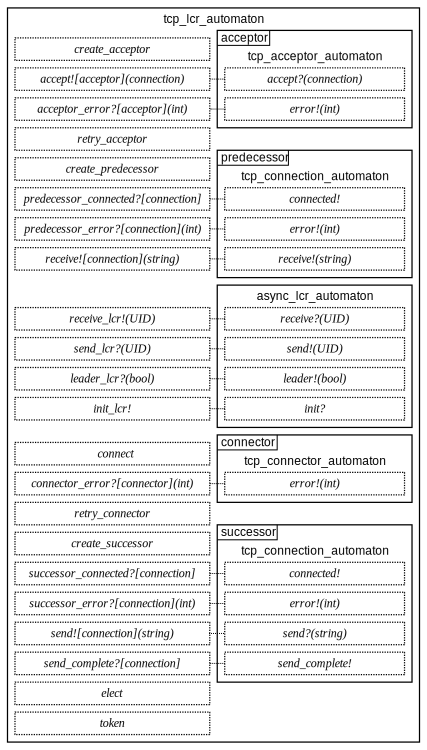
\includegraphics[width=\textwidth]{tcp_lcr_automaton}
\caption{TCP LCR automaton.}
\label{tcp_lcr_automaton}
\end{figure}

\paragraph{Leader election in a ring using TCP.}
The \verb+asynch_lcr_automaton+ is a reusable component designed to be used in the context of a larger system.
The \verb+tcp_lcr_automaton+ listed in \verb+examples/tcp_lcr.cpp+ elects a leader in a dynamic ring of processes.
The structure of the \verb+tcp_lcr_automaton+ is given in Figure~\ref{tcp_lcr_automaton}.
The \verb+tcp_lcr_automaton+ is composed with a \verb+tcp_acceptor_automaton+ to accept a connection from its predecessor, a \verb+tcp_connector_automaton+ to create a connection to its successor, and two \verb+tcp_connection_automaton+ representing the predecessor and successor, and a \verb+asynch_lcr_automaton+ to realize the leader election algorithm.
The leader of the ring periodically sends a token which is forwarded by all nodes in the ring.
If a node has not received a token for a specified duration of time, it calls for an election.
The \verb+asynch_lcr_automaton+ of Figure~\ref{tcp_lcr_automaton} can be substituted with a different automaton to realize a different leader election protocol or a different protocol altogether.

\paragraph{Binding predicates.}
The binding predicate supplied by ioa++ is the \verb+ioa::binding_count+ function which returns the number of actions bound to the specified actions.
The value returned by \verb+ioa::binding_count+ is zero for internal actions, one or zero for input actions, and non-negative for output actions.
Most often, \verb+ioa::binding_count+ is used in the precondition of outputs to ensure that the value generated by the output will be received.
This type of usage can be seen in the send action of the \verb+tcp_lcr_automaton+:
\begin{lstlisting}
  bool send_precondition (
    ioa::automaton_manager<ioa::tcp_connection_automaton>* s) const
 {
    return s == m_successor &&
           m_successor_connected &&
           m_clear_to_send && !m_send.empty () &&
           ioa::binding_count (&tcp_lcr_automaton::send, s) != 0;
  }
\end{lstlisting}

\paragraph{Dynamic composition.}
Dynamic composition is accomplished by creating child automata and binding to them.
The \verb+tcp_lcr_automaton+ creates a \verb+asynch_lcr_automaton+ and binds to it with the following code:
\begin{lstlisting}
    ioa::automaton_manager<asynch_lcr_automaton<uuid> >* lcr =
       ioa::make_automaton_manager (this,
         ioa::make_generator<asynch_lcr_automaton<uuid> > (m_u));
    ioa::make_binding_manager (this,
			       lcr, &asynch_lcr_automaton<uuid>::send,
			       &m_self, &tcp_lcr_automaton::send_lcr);
    ioa::make_binding_manager (this,
			       &m_self, &tcp_lcr_automaton::receive_lcr,
			       lcr, &asynch_lcr_automaton<uuid>::receive);
    ioa::make_binding_manager (this,
			       lcr, &asynch_lcr_automaton<uuid>::leader,
			       &m_self, &tcp_lcr_automaton::leader_lcr);
    ioa::make_binding_manager (this,
			       &m_self, &tcp_lcr_automaton::init_lcr,
			       lcr, &asynch_lcr_automaton<uuid>::init);
\end{lstlisting}
Children automata are managed by \verb+ioa::automaton_manager+ objects which can be created via the \verb+ioa::make_automaton_manager+ function.
An automaton manager object requires an \verb+ioa::automaton+ object for its system action implementation and a generator for allocating the child automaton.
Bindings are managed by \verb+ioa::binding_manager+ objects which can created via the \verb+ioa::make_binding_manager+ function.
A binding manager objects requires an \verb+ioa::automaton+ object for its system action implementation, a manager object for the output automaton, a reference to the output action, a manger object for the input automaton, a reference to the input action, and parameters for the actions if required.
The \verb+m_self+ object of the example is a \verb+ioa::handle_manager+ which can be used to bind to automata that already exist.
From the example, the \verb+tcp_lcr_automaton+ binds the \verb+asynch_lcr_automaton+ to itself.

\subsection{Building Real Systems}



%% Conclude with our recommendations for programming, highlight need for exploration.

%% Tips for Writing Programs with I/O Automata
%% 1. Make sure that a parameter exists.
%% 2. Move logic in observe to local actions.
%% 3. Avoid observing an arbitrary number of managers.
%% 4. Do not bind to managers allocated on the stack.
%% 5. Stop when an error is encoutered and report it.
%% 6. Make sure output actions are bound.
%% 7. Make sure local actions are scheduled.
%% 8. Do not pass pointers---use const_shared_ptr.
%% 9. Check preconditions.
%% 10. Check effects.
%% 11. Order clauses of preconditions for efficiency.
%% 12. Automata that should be destroyed at the same time should be created at the same time and vice versa.  (Group using a parent.)

%% \begin{outline}
%% \item State
%%   \begin{outline}
%%   \item There is no shared state in a 
%%   \item Local state only
%%   \item Shared state
%%     \begin{outline}
%%       \item Impossible in distributed systems
%%       \item Dangerous in local systems
%%     \end{outline}
%%   \end{outline}
%% \item Communication
%%   \begin{outline}
%%   \item Atomic asynchronous message passing
%%   \item Network sets size of atom (UDP)
%%   \item Can build reliable streams (TCP)
%%   \item Local equivalent is passing a value
%%   \item Model should lend itself to writing protocols
%%   \end{outline}
%% \item Asynchrony
%%   \begin{outline}
%%     \item Model must have natural support for asynchrony, i.e., event-based
%%     \item Leads to a more efficient implementation because changed state and enabled actions become obvious
%%   \end{outline}
%% \item Concurrency
%%   \begin{outline}
%%     \item Reason about systems using non-deterministic interleaving of atomic actions
%%     \item Model should admit implementations that execute concurrently
%%   \end{outline}
%% \item Dynamics
%%   \begin{outline}
%%     \item Configuration - Edges in graph of communicating components can change at run-time.
%%       \begin{outline}
%%       \item Already required in distributed settings
%%       \item Not addressed in formal models
%%       \end{outline}
%%     \item Extension - Nodes in graph of communicating components can change at run-time.
%%   \end{outline}
%%   \item Reflection
%% \end{outline}

%% I/O Automata
%% \begin{itemize}
%%   \item Compare with UNITY
%%   \item Compare with esterel
%%   \item Compare with pi calculus
%%   \item Compare with Ptolemy
%% \end{itemize}
